\documentclass[12pt]{beamer}
\usepackage{../Estilos/BeamerFC}
\usepackage{../Estilos/ColoresLatex}
\input{../Preambulos/pre_codigo}
\usepackage[siunitx]{circuitikz}
\usetikzlibrary{arrows,patterns,shapes}
\usetikzlibrary{decorations.markings}
\usetikzlibrary{arrows}
\input{../Preambulos/preambulo_Beamer_Copenhagen_wolverine}
\usefonttheme{serif}

\title{\large{EDO con CDF de orden superior}}
\subtitle{Tema 3 - Ecuaciones Diferenciales Ordinarias}
\author{M. en C. Gustavo Contreras Mayén}
\date{}

\begin{document}
\maketitle

\section*{Contenido}
\frame{\tableofcontents[currentsection, hideallsubsections]}

\section{ED de orden 4}
\frame{\tableofcontents[currentsection, hideothersubsections]}
\subsection{El problema}

\begin{frame}
\frametitle{Tipo particular de problema}
En aras de la brevedad, limitamos nuestra discusión al caso especial donde $\pderivada{y}$ e $\tderivada{y}$ no aparecen explícitamente en la ED, es decir, consideramos:
\pause
\begin{align*}
\nderivada{y}{4} = f (x, y, \sderivada{y})
\end{align*}
\pause 
Suponemos que se indican dos CDF en cada extremo del dominio de solución $(a, b)$. \pause Los problemas de este tipo se encuentran comúnmente en la teoría de vigas.
\end{frame}
\begin{frame}
\frametitle{Manera de abordar el problema}
Nuevamente dividimos el dominio de la solución en $m$ intervalos de longitud $h$ cada uno.
\\
\bigskip
\pause
Reemplazando las derivadas de $y$ por diferencias finitas en los puntos de malla, obtenemos las ecuaciones en diferencias finitas:
\end{frame}
\begin{frame}
\frametitle{Sistema de ecuaciones}
\begin{align}
\dfrac{y_{i-2} {-} 4 \, y_{i-1} {+} 6 \, y_{i} {-} 4 \, y_{i+1} {+} y_{i+2}}{h^{4}} = f \bigg( x_{i}, y_{i}, \dfrac{y_{i-1} {-} 2 \, y_{i} {+} y_{i+1}}{h^{2}} \bigg)
\label{eq:ecuacion_08_12}
\end{align}
con $i = 0, 1, \ldots, m$
\end{frame}
\begin{frame}
\frametitle{De manera explícita}
\begin{subequations}
\begin{align}
&{} \hspace*{-2cm} \begin{aligned}[b]
y_{-2} - 4 \, y_{-1} &+ 6 \, y_{0} - 4 \, y_{1} + y_{2} + \\
&- h^{4} \, f \bigg( x_{0}, y_{0}, \dfrac{y_{-1} {-} 2 \, y_{0} {+} y_{1}}{h^{2}} \bigg) = 0
\end{aligned}
\label{eq:ecuacion_08_13a} \\ 
&{} \hspace*{-2cm} \begin{aligned}[b]
y_{-1} {-} 4 \, y_{0} &+ 6 \, y_{1} - 4 \, y_{2} + y_{3} + \\
&- h^{4} \, f \bigg( x_{1}, y_{1}, \dfrac{y_{0} {-} 2 \, y_{1} {+} y_{2}}{h^{2}} \bigg) = 0
\end{aligned}
\label{eq:ecuacion_08_13b} \\ 
&{} \hspace*{-2cm} \begin{aligned}[b]
y_{0} - 4 \, y_{1} &+ 6 \, y_{2} - 4 \, y_{3} + y_{4} + \\
&- h^{4} \, f \bigg( x_{2}, y_{2}, \dfrac{y_{1} {-} 2 \, y_{2} {+} y_{3}}{h^{2}} \bigg) = 0
\end{aligned}
\label{eq:ecuacion_08_13c}
\end{align} 
\end{subequations}
\end{frame}
\begin{frame}
\frametitle{De manera explícita}
\begin{subequations}
\begin{align}
\vdots \nonumber \\
&{} \hspace*{-1cm} \begin{aligned}[b] 
y_{m-3} - 4 \, y_{m-2} &+ 6 \, y_{m-1} - 4 \, y_{m} + y_{m+1} + \\
&- h^{4} \, f \bigg( x_{m-1}, y_{m-1}, \dfrac{y_{m-2} {-} 2 \, y_{m-1} {+} y_{m}}{h^{2}} \bigg) = 0
\end{aligned}
\label{eq:ecuacion_08_13d} \tag{2d} \\
&{} \hspace*{-1cm} \begin{aligned}[b]
y_{m-2} - 4 \, y_{m-1} &+ 6 \, y_{m} - 4 \, y_{m+1} + y_{m+2} + \\
&- h^{4} \, f \bigg( x_{m}, y_{m}, \dfrac{y_{m-1} {-} 2 \, y_{m} {+} y_{m+1}}{h^{2}} \bigg) = 0
\end{aligned}
\label{eq:ecuacion_08_13e} \tag{2e}
\end{align} 
\end{subequations}
\end{frame}
\begin{frame}
\frametitle{Puntos adicionales}
Ahora vemos que hay cuatro incógnitas: $y_{-2}, y_{-1}, y_{m+1}$ y $y_{m+2}$ que se encuentran fuera del dominio de la solución y deben eliminarse aplicando las CDF, una tarea que facilita la siguiente tabla.
\end{frame}
\begin{frame}
\frametitle{Tabla para los puntos adicionales y CDF}
\begin{table}
\centering
\begin{tabular}{c | l}
CDF & Expresión en diferencias finitas equivalente \\ \hline
$y (a) = \alpha$ & $y_{0} = \alpha$ \\ \hline
$\pderivada{y} (a) = \alpha$ & $y_{-1} = y_{1} - 2 \, h \, \alpha$ \\ \hline
$\sderivada{y} (a) = \alpha$ & $y_{-1} = 2 \, y_{0} - y_{1} + h^{2} \, \alpha$ \\ \hline
$\tderivada{y} (a) = \alpha$ & $y_{-2} = 2 \, y_{-1} - 2 \, y_{1} + y_{2} - 2 \, h^{3} \, \alpha$ \\ \hline
\end{tabular}
\end{table}
\end{frame}
\begin{frame}
\frametitle{Tabla para los puntos adicionales y CDF}
\begin{table}
\centering
\begin{tabular}{c | l}
CDF & Expresión en diferencias finitas equivalente \\ \hline
$y (b) = \beta$ & $y_{m} = \beta$ \\ \hline
$\pderivada{y} (b) = \beta$ & $y_{m+1} = y_{m-1} - 2 \, h \, \beta$ \\ \hline
$\sderivada{y} (b) = \beta$ & $y_{m+1} = 2 \, y_{m} - y_{m-1} + h^{2} \, \beta$ \\ \hline
$\tderivada{y} (b) = \beta$ & $y_{m+2} = 2 \, y_{m+1} - 2 \, y_{m-1} + y_{m-22} - 2 \, h^{3} \, \beta$ \\ \hline
\end{tabular}
\end{table}
\end{frame}
\begin{frame}
\frametitle{Combinaciones con sentido}
El observador astuto puede notar que algunas combinaciones de las CDF no funcionarán para eliminar el \enquote{exceso}.
\\
\bigskip
\pause
Una de esas combinaciones es claramente \pause $y (a) = \alpha_{1}$ e $\tderivada{y} (a) = \alpha_{2}$. \pause Otra
 combinación es $\pderivada{y} (a) = \alpha_{1}$ e $\sderivada{y} (a) = \alpha_{2}$.
\end{frame}
\begin{frame}
\frametitle{Congruencia con la física}
En el contexto de la teoría de vigas, esto tiene sentido:
\pause
\setbeamercolor{item projected}{bg=bananayellow,fg=cerise}
\setbeamertemplate{enumerate items}{%
\usebeamercolor[bg]{item projected}%
\raisebox{1.5pt}{\colorbox{bg}{\color{fg}\footnotesize\insertenumlabel}}%
}
\begin{enumerate}[<+->]
\item Podemos imponer un desplazamiento $y$ o una fuerza cortante $E \, I \,  \tderivada{y}$ en un punto.
\item Pero es imposible aplicar ambos simultáneamente.
\end{enumerate}
\end{frame}
\begin{frame}
\frametitle{Congruencia con la física}
De manera similar, \pause no tiene sentido físico indicar tanto la pendiente $\pderivada{y}$ como el momento de flexión $E \, I \, \sderivada{y}$ en el mismo punto.
\end{frame}

\subsection{Ejercicio 1}

\begin{frame}
\frametitle{Enunciado del Ejercicio}
Una viga uniforme de longitud $L$ y rigidez a la flexión $E \, I$ está unida a soportes rígidos en ambos extremos.
\\
\bigskip
\pause
\begin{figure}
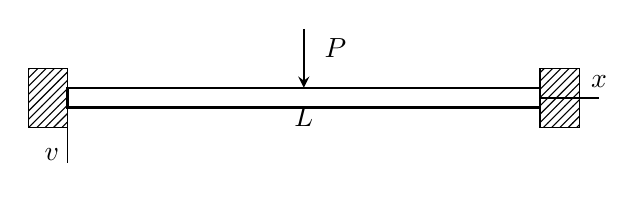
\begin{tikzpicture}
    \draw [thick] (0, 0) rectangle (6, 0.25) node [midway, below] {$L$};
    \draw [-stealth, thick] (3, 1) -- (3, 0.25);
    \node at (3.4, 0.75) {$P$};
    \draw [pattern= north east lines] (0, -0.25) rectangle (-0.5, 0.5);
    \draw [pattern= north east lines] (6, -0.25) rectangle (6.5, 0.5);
    \draw [thick] (6, 0.12) -- (6.75, 0.12) node [above, near end, pos=1] {$x$};
    \draw (0, 0) -- (0, -0.7);
    \node at (-0.2, -0.6) {$v$};
\end{tikzpicture}
\end{figure}
\end{frame}
\begin{frame}
\frametitle{Enunciado del problema}
La viga soporta una carga concentrada $P$ en la mitad de su longitud.
\\
\bigskip
\pause
Si utilizamos simetría y modelamos solo la mitad izquierda de la viga, el desplazamiento $v$ se puede obtener resolviendo el problema de CDF:
\end{frame}
\begin{frame}
\frametitle{Ecuación para la viga}
\begin{align*}
&E \, I \, \dv[4]{v}{x} = 0 \\[1em]
&v \eval_{x=0} = 0, \hspace{1cm} \dv{v}{x} \eval_{x=0} = 0 \\[1em]
&\dv{v}{x} \eval_{x=\frac{L}{2}} = 0 \hspace{1cm} E \, I \, \dv[3]{v}{x} \eval_{x=\frac{L}{2}} = -\dfrac{P}{2}
\end{align*}
\end{frame}
\begin{frame}
\frametitle{Problema a resolver}
Utiliza el método de diferencias finitas para determinar el desplazamiento y el momento de flexión:
\begin{align*}
M = - E \, I \, \dv[2]{v}{x}
\end{align*}
en la mitad de la viga.
\end{frame}
\begin{frame}
\frametitle{Haciendo un cambio de variables}
Usamos las siguientes variables adimensionales:
\\
\bigskip
\pause
\begin{align*}
\xi = \dfrac{x}{L} \hspace{1.5cm} y = \dfrac{E \, I}{P \, L^{3}} \, v
\end{align*}
\end{frame}
\begin{frame}
\frametitle{Reexpresando el problema}
El problema pasa a ser:
\pause
\begin{align*}
&\dv[4]{v}{\xi} = 0 \\[1em]
&y \eval_{\xi=0} = 0, \hspace{1cm} \dv{y}{\xi} \eval_{x=0} = 0 \\[1em]
&\dv{y}{\xi} \eval_{x=\frac{1}{2}} = 0 \hspace{1cm} \dv[3]{y}{\xi} \eval_{x=\frac{1}{2}} = -\dfrac{1}{2}
\end{align*}    
\end{frame}
\begin{frame}
\frametitle{Escribiendo las ecuaciones}
Ahora procedemos a escribir las ecs. (2), teniendo en cuenta las CDF.
\\
\bigskip
\pause
Usando la tabla anterior, las expresiones de diferencias finitas de las CDF en el extremo izquierdo son $y_{0} = 0$ e $y_{-1} = y_{1}$.
\end{frame}
\begin{frame}
\frametitle{Revisando las ecuaciones}
Por lo tanto, las ecs. (\ref{eq:ecuacion_08_13a}) y (\ref{eq:ecuacion_08_13b}) se convierten en:
\pause
\begin{subequations}
\begin{align}
y_{0} =& 0 \label{eq:ecuacion_a} \tag{a} \\
- 4 \, y_{0} + 7 \, y_{1} - 4 \, y_{2} + y_{3} =& 0 \label{eq:ecuacion_b} \tag{b}
\end{align}
\end{subequations}
\end{frame}
\begin{frame}
\frametitle{Revisando las ecuaciones}
La ec. (\ref{eq:ecuacion_08_13c}) es:
\pause
\begin{align}
y_{0} - 4 \, y_{1} + 6 \, y_{2} - 4 \, y_{3} + y_{4} = 0 \label{eq:ecuacion_c} \tag{c}
\end{align}
\end{frame}
\begin{frame}
\frametitle{Revisando las ecuaciones}
Al lado derecho las CDF son equivalentes a $y_{m+1} = y_{m-1}$ y
\begin{align*}
y_{m+2} = 2 \, y_{m+1} + y_{m-2} - 2 \, y_{m-1} + 2 \, h^{3} (-1/2) = y_{m-2} - h^{3}
\end{align*}
\end{frame}
\begin{frame}
\frametitle{Revisando las ecuaciones}
Al sustituir en las ecs. (\ref{eq:ecuacion_08_13d}) y (\ref{eq:ecuacion_08_13e}), se tiene:
\pause
\begin{subequations}
\begin{align}
y_{m-3} - 4 \, y_{m-2} + 7 \, y_{m-1} - 4 \, y_{m} = 0 \label{eq:ecuacion_d} \tag{d} \\[0.5em]
2 \, y_{m-2} - 8 \, y_{m-1} + 6 \, y_{m} = h^{3} \label{eq:ecuacion_e} \tag{e}
\end{align}
\end{subequations}
\end{frame}
\begin{frame}
\frametitle{La matriz de coeficientes}
La matriz de coeficientes de las ecs. (\ref{eq:ecuacion_a}) - (\ref{eq:ecuacion_d}) se puede hacer simétrica \pause dividiendo la ec. (\ref{eq:ecuacion_e}) entre $2$.
\end{frame}
\begin{frame}
\frametitle{Matriz de coeficientes}
\renewcommand{\arraystretch}{1}
\begin{align*}
\begin{bmatrix}
1 & 0 & 0 & & & & & \\
0 & 7 & -4 & 1 & & & & \\
0 & -4 & 6 & -4 & 1 & & & \\
 & \ddots & \ddots & \ddots & \ddots & \ddots & & \\
 & & 1 & -4 & 6 & -4 & 1 \\
 & & & 1 & -4 & 7 & -4 \\
 & & & & 1 & -4 & 3
\end{bmatrix}
\begin{bmatrix}
y_{0} \\
y_{1} \\
y_{2} \\
\vdots \\
y_{m-2} \\
y_{m-1} \\
y_{m}
\end{bmatrix}
=
\begin{bmatrix}
0 \\
0 \\
0 \\
\vdots \\
0 \\
0 \\
0.5 h^{3} \\
\end{bmatrix}
\end{align*}
\end{frame}
\begin{frame}
\frametitle{Matriz de coeficientes resultante}
Hemos llegado a una matriz simétrica con $5$ diagonales, \pause también conocida como \textbf{\textcolor{ao}{matriz pentadiagonal}}.
\\
\bigskip
\pause
Tendremos que hacer una revisión sobre cómo resolver estas matrices, tal como lo hicimos con las matrices triadiagonales.
\end{frame}

\section{Matrices Coeficientes Simétricos}
\frame{\tableofcontents[currentsection, hideothersubsections]}
\subsection{Propiedades}

\begin{frame}
\frametitle{Matrices de coeficientes}
La mayoría de las veces, las matrices de coeficientes que surgen en los problemas de ingeniería son tanto simétricas como en banda.
\\
\bigskip
\pause
Por lo tanto, vale la pena descubrir las propiedades especiales de tales matrices y aprender a usarlas en la construcción de algoritmos eficientes.
\end{frame}
\begin{frame}
\frametitle{Manejando una matriz simétrica}
Si la matriz $\textbf{A}$ es simétrica, \pause entonces la descomposición $\mathbf{L \, U}$ se puede presentar en la forma:
\pause
\begin{align}
\mathbf{A} = \mathbf{L \, U} = \mathbf{L \, D} \, \mathbf{L}^{T}
\label{eq:ecuacion_02_23} 
\end{align}
donde $\mathbf{D}$ es una matriz diagonal.
\end{frame}
\begin{frame}
\frametitle{La descomposición de Choleski}
Un ejemplo es la descomposición de Choleski $\mathbf{A} = \mathbf{L \, L}^{T}$ que se discutió anteriormente (para ese caso $\mathbf{D} = \mathbf{I}$)
\end{frame}
\begin{frame}
\frametitle{Descompsición Doolittle}
Para la descomposición Doolittle se tiene que:
\pause
\renewcommand{\arraystretch}{0.8}
\begin{align*}
&\mathbf{U} = \mathbf{D \, L}^{T} = \\
&=
\begin{bmatrix}
D_{1} & 0 & 0 & \ldots & 0 \\
0 & D_{2} & 0 & \ldots & 0 \\
0 & 0 & D_{3} & \ldots & 0 \\
\vdots & \vdots & \vdots & \ldots & \vdots \\
0 & 0 & 0 & \ldots & D_{n}
\end{bmatrix}
\begin{bmatrix}
1 & L_{21} & L_{31} & \ldots & L_{n1} \\
0 & 1 & L_{32} & \ldots & L_{n2} \\
0 & 0 & 1 & \ldots & L_{n3} \\
\vdots & \vdots & \vdots & \ldots & \vdots \\
0 & 0 & 0 & \vdots & 1
\end{bmatrix}
\end{align*}
\end{frame}
\begin{frame}
\frametitle{La matriz $\mathbf{U}$}
Lo que nos devuelve:
\pause
\renewcommand{\arraystretch}{0.9}
\begin{align}
\mathbf{U} =
\begin{bmatrix}
D_{1} & D_{1} L_{21} & D_{1} L_{31} & \ldots & D_{1} L_{n1} \\
0 & D_{2} & D_{2} L_{32} & \ldots & D_{2} L_{n2} \\
0 & 0 & D_{3} & \ldots & D_{3} L_{n3} \\
\vdots & \vdots & \vdots & \ldots & \vdots \\
0 & 0 & 0 & \ldots & D_{n}
\end{bmatrix}
\label{eq:ecuacion_02_24}
\end{align}
\end{frame}
\begin{frame}
\frametitle{Matrices que se almacenan}
Ahora vemos que durante la descomposición de una matriz simétrica solo se debe almacenar $\mathbf{U}$, porque $\mathbf{D}$ y $\mathbf{L}$ se pueden recuperar fácilmente de $\mathbf{U}$.
\end{frame}
\begin{frame}
\frametitle{Matriz triangular superior}
Por lo tanto, la eliminación de Gauss, que da como resultado una matriz triangular superior de la forma que se muestra en la ec. (\ref{eq:ecuacion_02_24}), es suficiente para descomponer una matriz simétrica.
\end{frame}
\begin{frame}
\frametitle{Esquema alternativo}
Existe un esquema de almacenamiento alternativo que se puede emplear durante la descomposición de $\mathbf{LU}$. \pause La idea es llegar a la matriz:
\renewcommand{\arraystretch}{0.9}
\begin{align}
\mathbf{U}^{*} =
\begin{bmatrix}
D_{1} & L_{21} & L_{31} & \ldots & L_{n1} \\
0 & D_{2} & L_{32} & \ldots & L_{n2} \\
0 & 0 & D_{3} & \ldots & L_{n3} \\
\vdots & \vdots & \vdots & \ldots & \vdots \\
0 & 0 & 0 & \ldots & D_{n}
\end{bmatrix}
\label{eq:ecuacion_02_25}
\end{align}
\end{frame}
\begin{frame}
\frametitle{Solución más eficiente}
Aquí $\mathbf{U}$ se puede recuperar de $U_{ij} = D_{i} \, L_{ji}$.
\\
\bigskip
\pause
Resulta que este esquema conduce a una fase de solución computacionalmente más eficiente; \pause por lo tanto, lo adoptamos para matrices simétricas con bandas.
\end{frame}

\section{Matrices pentadiagonales}
\frame{\tableofcontents[currentsection, hideothersubsections]}
\subsection{Estudiando la matriz}

\begin{frame}
\frametitle{Matrices pentadiagonales}
Encontramos matrices pentadiagonales de coeficientes (\textbf{\textcolor{cadet}{ancho de banda}} = $5$) en la solución de ED4 por diferencias finitas. A menudo, estas matrices son simétricas, en cuyo caso una matriz de coeficientes $n \times n$ tiene la forma:
\end{frame}
\begin{frame}
\frametitle{Matrices pentadiagonales}
\renewcommand{\arraystretch}{0.9}
\begin{align}
\mathbf{A} =
\begin{bmatrix}
d_{1} & e_{1} & f_{1} & 0 & 0 & 0 & \ldots & 0 \\
e_{1} & d_{2} & e_{2} & f_{2} & 0 & 0 & \ldots & 0 \\
f_{1} & e_{2} & d_{2} & e_{3} & f_{3} & 0 & \ldots & 0 \\
0 & f_{2} & e_{3} & d_{4} & e_{4} & f_{4} & \ldots & 0 \\
\vdots & \vdots & \vdots & \vdots & \vdots & \vdots \ddots & \vdots \\
0 & \ldots & 0 & f_{n-4} & e_{n-3} & d_{n-2} & e_{n-2} &f_{n-2} \\
0 & \ldots & 0 & 0 & f_{n-3} & e_{n-2} & d_{n-1} & e_{n-1} \\
0 & \ldots & 0 & 0 & 0 & f_{n-2} & e_{n-1} & d_{n}
\end{bmatrix}
\label{eq:ecuacion_02_26}
\end{align}
\end{frame}
\begin{frame}
\frametitle{Vectores columna}
Como en el caso de las matrices tridiagonales, se almacenan los elementos no nulos en tres vectores:
\pause
\renewcommand{\arraystretch}{0.9}
\begin{align*}
\mathbf{d} = \begin{bmatrix}
d_{1} \\
d_{2} \\
\vdots \\
d_{n-2} \\
d_{n-1} \\
d_{n}
\end{bmatrix}
\hspace{1.3cm}
\mathbf{e} =
\begin{bmatrix}
e_{1} \\
e_{2} \\
\vdots \\
e_{n-2} \\
e_{n-1}
\end{bmatrix}
\hspace{1.3cm}
\mathbf{f} =
\begin{bmatrix}
f_{1} \\
f_{2} \\
\vdots \\
f_{n-2}
\end{bmatrix}
\end{align*}
\end{frame}
\begin{frame}
\frametitle{Fase de solución}
Veamos ahora la solución de las ecuaciones $\mathbf{A \, x} = \mathbf{b}$ por la descomposición de Doolittle.
\\
\bigskip
\pause
El primer paso es transformar $\mathbf{A}$ a la forma triangular superior por eliminación de Gauss. \pause Si la eliminación ha progresado hasta la etapa en la que la k-ésima fila se ha convertido en la fila pivote, tenemos la siguiente situación:
\end{frame}
\begin{frame}
\frametitle{Renglón pivote}
\renewcommand{\arraystretch}{0.9}
\begin{align*}
\mathbf{A} =
\left[
\begin{array}{c c | c c c | c c c c}
\ddots & \vdots & \vdots & \vdots & \vdots & \vdots & \vdots & \vdots & \\ \hline
\ldots & 0 & d_{k} & e_{k} & f_{k} & 0 & 0 & 0 & \vdots \\
\ldots & 0 & e_{k} & d_{k+1} & e_{k+1} & f_{k+1} & 0 & 0 & \vdots \\
\ldots & 0 & f_{k} & e_{k+1} & d_{k+2} & e_{k+2} & f_{k+2} & 0 & \vdots \\ \hline
\ldots & 0 & 0 & f_{k+1} & e_{k+2} & d_{k+3} & e_{k+3} & f_{k+3} & \vdots \\
 & \vdots & \vdots & \vdots & \vdots & \vdots & \vdots & \vdots & \ddots
\end{array}
\right]
\end{align*}
\end{frame}
\begin{frame}
\frametitle{Aplicando operaciones elementales}
Los elementos $e_{k}$ y $f_{k}$ por debajo del renglón pivote (el k-ésimo renglón) se eliminan por las operaciones:
\pause
\begin{align*}
\text{renglón } (k + 1) \leftarrow \text{renglón } (k + 1) - (e_{k}/d_{k}) \times \text{renglón } k \\[0.5em]
\text{renglón } (k + 2) \leftarrow \text{renglón } (k + 2) - (f_{k}/d_{k}) \times \text{renglón } k
\end{align*}
\end{frame}
\begin{frame}
\frametitle{Términos que se modifican}
Los únicos términos (aparte de los que están siendo eliminados) que son cambiados por las operaciones son:
\pause
\begin{align}
\begin{aligned}
d_{k+1} \leftarrow d_{k+1} - (e_{k}/d_{k}) \, e_{k} \\[0.5em]
e_{k+1} \leftarrow e_{k+1} - (e_{k}/d_{k}) \, f_{k} \\[0.5em]
d_{k+2} \leftarrow d_{k+2} - (f_{k}/d_{k}) \, f_{k}
\end{aligned}
\label{eq:ecuacion_02_27a}
\end{align}
\end{frame}
\begin{frame}
\frametitle{Almacenando los multiplicadores}
Guardando los multiplicadores en la porción triagular superior de la matriz de resultado en:
\pause
\begin{align}
e_{k} \leftarrow e_{k}/d_{k} \hspace{2cm} f_{k} \leftarrow f_{k}/d_{k}
\label{eq:ecuacion_02_27b}
\end{align}
\end{frame}
\begin{frame}
\frametitle{Terminando fase de eliminación}
Al final de la fase de eliminación, la matriz tiene la forma (no confundir $\mathbf{d}$, $\mathbf{e}$ y $\mathbf{f}$ con el contenido original de $\mathbf{A}$):
\pause
\renewcommand{\arraystretch}{0.9}
\begin{align*}
\mathbf{U}^{*} =
\begin{bmatrix}
d_{1} & e_{1} & f_{1} & 0 & \ldots & 0 \\
0 & d_{2} & e_{2} & f_{2} & \ldots & 0 \\
0 & 0 & d_{3} & e_{3} & \ldots & 0 \\
\vdots & \vdots & \vdots & \vdots & \ldots & \vdots \\
0 & 0 & \ldots & 0 & d_{n-1} & e_{n-1} \\
0 & 0 & \ldots & 0 & 0 & d_{n} \\
\end{bmatrix}
\end{align*}
\end{frame}
\begin{frame}
\frametitle{Fase de solución}
El siguiente paso es implementar la fase de solución.
\\
\bigskip
\pause
Las ecuaciones $\mathbf{L \, y} =  \mathbf{b}$ tiene la matriz aumentada de coeficientes:
\end{frame}
\begin{frame}
\frametitle{La matriz aumentada}
\renewcommand{\arraystretch}{0.9}
\begin{align*}
\big[ \mathbf{L} \vert \mathbf{b} \big] = 
\left[
\begin{array}{c c c c c c | c}
1 & 0 & 0 & 0 & \ldots & 0 & b_{1} \\
e_{1} & 1 & 0 & 0 & \ldots & 0 & b_{2} \\
f_{1} & e_{2} & 1 & 0 & \ldots & 0 & b_{3} \\
0 & f_{2} & e_{3} & 1 & \ldots & 0 & b_{4} \\
\vdots & \vdots & \vdots & \vdots & \ldots & \vdots & \vdots \\
0 & 0 & 0 & f_{n-2} & e_{n-1} & 1 & b_{n}
\end{array}
\right]
\end{align*}
\end{frame}
\begin{frame}
\frametitle{Sustitución hacia adelante}
Resolviendo hacia adelante, llegamos a:
\pause
\begin{align}
\begin{aligned}
y_{1} &= b_{1} \\[0.5em]
y_{2} &= b_{2} - e_{1} \, y_{1} \\[0.5em]
&\vdots \\
y_{k} &= b_{k} - f_{k-2} \, y_{k-2} - e_{k-1} \, y_{k-1}
\end{aligned}
\label{eq:ecuacion_02_28}
\end{align}
\end{frame}
\begin{frame}
\frametitle{Sustitución hacia atrás}
Estas ecuaciones se resuelven hacia atrás, \pause llamemos $\mathbf{U \, x} = \mathbf{y}$, que contiene la matriz aumentada:
\pause
\renewcommand{\arraystretch}{0.9}
\begin{align*}
\big[ \mathbf{U} \vert \mathbf{y} \big] = 
\left[
\begin{array}{c c c c c c | c}
d_{1} & d_{1} e_{1} & d_{1} f_{1} & 0 & \ldots & 0 & y_{1} \\
0 & d_{2} & d_{2} e_{2} & d_{2} f_{2} & \ldots & 0 & y_{2} \\
0 & 0 & d_{3} & d_{3} e_{3} & \ldots & 0 & y_{3} \\
\vdots & \vdots & \vdots & \vdots & \ldots & \vdots & \vdots \\
0 & 0 & \ldots & 0 & d_{n-1} & d_{n-1} e_{n-1} & y_{n-1} \\
0 & 0 & \ldots & 0 & 0 & d_{n} & y_{n}
\end{array}
\right]
\end{align*}
\end{frame}
\begin{frame}
\frametitle{Solución al sistema}
La solución se obtiene por sustitución hacia atrás:
\pause
\begin{align*}
x_{n} &= y_{n} / d_{n} \\[0.5em]
x_{n-1} &= y_{n-1} / d_{n-1} - e_{n-1} \\[0.5em]
x_{n}& = \vdots \\[0.5em]
x_{k} &= y_{k} / d_{k} - e_{k} x_{k+1} - f_{k} x_{k+2} \\[0.5em]
k &= n - 2, n - 3, \ldots, 1
\end{align*}
\end{frame}

\subsection{La función \texttt{LUdescomp5}}

\begin{frame}
\frametitle{Código en \python}
Se presenta el código en \python{} de la función \funcionazul{LUdescomp5} que descompone una matriz $\mathbf{A}$  simétrica y pentadiagonal de la forma $\mathbf{A} = [ \mathbf{f} \backslash \mathbf{e} \backslash \mathbf{d} \backslash \mathbf{e} \backslash \mathbf{f}]$.
\end{frame}
\begin{frame}
\frametitle{Reemplazando vectores}
Los vectores originales $\mathbf{d}, \mathbf{e}, \mathbf{f}$ se reemplazan por los vectores obtenidos por la descomposición de la matriz.
\\
\bigskip
\pause
Luego de la descomposición, la solución $\mathbf{A x} = \mathbf{b}$ se obtiene mediante la función \funcionazul{LUsoluc5}.
\end{frame}
\begin{frame}
\frametitle{Sustitución hacia adelante/atrás}
Durante la sustitución hacia adelante, el vector $\mathbf{b}$ original se reemplaza por $\mathbf{y}$.
\\
\bigskip
\pause
De manera similar, el vector $\mathbf{y}$ se sobrescribe con $\mathbf{x}$ en la fase de sustitución hacia atrás, de modo que el vector $\mathbf{b}$ contiene el vector solución al salir de \funcionazul{LUsoluc5}.
\end{frame}
\begin{frame}
\frametitle{Las funciones en \python}
Las siguientes funciones \funcionazul{LUdescomp5} y \funcionazul{LUsoluc5} deben de incluirse en el módulo \funcionazul{moduloMatrices}.
\end{frame}
\begin{frame}[allowframebreaks, fragile]
\frametitle{Las funciones en \python}
\begin{lstlisting}[caption=Funciones para resolver una matriz simétrica y pentadiagonal]
def LUdescomp5(d, e, f):
    n = len(d)
    
    for k in range(n-2):
        lam = e[k]/d[k]
        d[k+1] = d[k+1] - lam * e[k]
        e[k+1] = e[k+1] - lam * f[k]
        e[k] = lam
        lam = f[k]/d[k]
        d[k+2] = d[k+2] - lam * f[k]
        f[k] = lam
        
    lam = e[n-2]/d[n-2]
    d[n-1] = d[n-1] - lam * e[n-2]
    e[n-2] = lam
    
    return d, e, f

def LUsoluc5(d, e, f, b):
    n = len(d)
    b[1] = b[1] - e[0] * b[0]
    
    for k in range(2, n):
        b[k] = b[k] - e[k-1] * b[k-1] - f[k-2] * b[k-2]
        
    b[n-1] = b[n-1]/d[n-1]
    b[n-2] = b[n-2]/d[n-2] - e[n-2] * b[n-1]
    
    for k in range(n-3, -1, -1):
        b[k] = b[k]/d[k] - e[k] * b[k+1] - f[k] * b[k+2]
    
    return b
\end{lstlisting}
\end{frame}

\section{Regresando al ejercicio}
\frame{\tableofcontents[currentsection, hideothersubsections]}
\subsection{Solución al problema}

\begin{frame}
\frametitle{¿En dónde nos quedamos?}
En el problema de la viga, llegamos al sistema:
\renewcommand{\arraystretch}{0.9}
\begin{align*}
\begin{bmatrix}
1 & 0 & 0 & & & & & \\
0 & 7 & -4 & 1 & & & & \\
0 & -4 & 6 & -4 & 1 & & & \\
 & \ddots & \ddots & \ddots & \ddots & \ddots & & \\
 & & 1 & -4 & 6 & -4 & 1 \\
 & & & 1 & -4 & 7 & -4 \\
 & & & & 1 & -4 & 3
\end{bmatrix}
\begin{bmatrix}
y_{0} \\
y_{1} \\
y_{2} \\
\vdots \\
y_{m-2} \\
y_{m-1} \\
y_{m}
\end{bmatrix}
=
\begin{bmatrix}
0 \\
0 \\
0 \\
\vdots \\
0 \\
0 \\
0.5 h^{3} \\
\end{bmatrix}
\end{align*}
\end{frame}
\begin{frame}
\frametitle{Solución con el código}
Que bien ahora podemos resolver con las funciones que recién mencionamos: \funcionazul{LUdescomp5} y \funcionazul{LUsoluc5}.
\end{frame}
\begin{frame}[allowframebreaks, fragile]
\frametitle{Código por completar}
\begin{lstlisting}[caption=Código para resolver el problema de la viga]
def ecuaciones(x, h, m):
    d = 
    e = 
    f = 
    b = 
    d[0] = 
    d[1] = 
    e[0] = 
    f[0] = 
    d[m-1] = 
    d[m] = 
    b[m] = 
    return d, e, f, b

xInicio = 0.0
xAlto = 0.5
m = 20
h = (xAlto - xInicio)/m

x = np.arange(xInicio,xAlto + h, h)

d, e, f, b = ecuaciones(x, h, m)

d, e, f = LUdescomp5(d, e, f)
y = LUsoluc5(d, e, f, b)

print('\n        x              y')
print('{0:14.5e} {1:14.5e}'.format(x[m-1], y[m-1]))
print('{0:14.5e} {1:14.5e}'.format(x[m], y[m]))
\end{lstlisting}
\end{frame}
\begin{frame}
\frametitle{Análisis de la solución}
Habiendo ejecutado el programa con $m = 20$, se tomaron la penúltima y última línea de la solución:
\begin{table}
\centering
\begin{tabular}{ | c| c |} \hline
$x$ & $y$ \\ \hline
$4.75000e-01$ & $5.19531e-03$ \\ \hline
$5.00000e-01$ & $5.23438e-03$ \\ \hline
\end{tabular}
\end{table}
\end{frame}
\begin{frame}
\frametitle{Análisis de la solución}
Por lo tanto, a la mitad de la viga tenemos que:
\pause
\begin{align*}
v \eval_{x=0.5 L} = \dfrac{P  \: L^{3}}{E \: I} \: y \eval_{\xi=0.5} = \num{5.23438d-3} \; \dfrac{P \: L^{3}}{E \: I}
\end{align*}
\pause
La solución exacta es:
\pause
\begin{align*}
v \eval_{x=0.5 L} = \num{5.20833d-3} \; \dfrac{P \: L^{3}}{E \: I}
\end{align*}
\end{frame}
\begin{frame}
\frametitle{Análisis de la solución}
Usamos los valores $m-1$ y $m$ de la solución que recuperamos con el código:
\pause
\begin{eqnarray*}
\begin{aligned}
\dv[2]{v}{x} \eval_{x=0.5 L} &= \pause \dfrac{P \: L^{3}}{E \: I} \left( \dfrac{1}{L^{2}} \: \dv[2]{y}{\xi} \eval_{\xi=0.5} \right) \, \simeq \\[0.5em] \pause 
&\simeq  \dfrac{P \: L}{E \: I} \: \dfrac{y_{m-1} - 2 y_{m} + y_{m+1}}{h^{2}} = \\[0.5em] \pause
&= \dfrac{P \: L}{E \: I} \dfrac{(5.19531 - 2(5.23438) + 5.19531) \times 10^{-3}}{0.025^{2}} = \\[0.5em] \pause
&= -0.125024 \: \dfrac{P \: L}{E \: I}
\end{aligned}
\end{eqnarray*}
\end{frame}
\begin{frame}
\frametitle{Análisis de la solución}
Ya podemos calcular el momento de flexión de la viga:
\pause
\begin{align*}
M \eval_{x=0.5 L} = - E \: I \: \dv[2]{v}{x} \eval_{\xi=0.5} = 0.125024 \: P \: L
\end{align*}
\pause
La solución exacta es:
\pause
\begin{align*}
M \eval_{x=0.5 \: L} = 0.125000 \: P \: L
\end{align*}
\end{frame}
\begin{frame}
\frametitle{Gráfica de la solución}
\begin{figure}
    \centering
    \includegraphics[scale=0.55]{Imagenes/plot_CDF_Dif_Fin_Ejercicio_02_01.eps}
\end{figure}
\end{frame}
\begin{frame}
\frametitle{Interpretación del resultado}
De la gráfica anterior encontramos que en el punto $x = 0.5 L$ se tiene un desplazamiento máximo de la viga.
\\
\bigskip
\pause
Al inicio del problema se comentó que debido a la simetría del problema, se simplificaba la solución para el punto medio de la barra, \pause por lo que podemos presentar el desplazamiento en toda la barra.
\end{frame}
\begin{frame}
\frametitle{Interpretación del resultado}
Haciendo un pequeño manejo en el arreglo \funcionazul{y} mediante \texttt{y[::-1]}, invertimos el orden de los elementos del arreglo.
\\
\bigskip
\pause
Quedando solo un ajuste para el dominio en $x$.
\end{frame}
\begin{frame}
\frametitle{Gráfica de la solución completa}
\begin{figure}
    \centering
    \includegraphics[scale=0.55]{Imagenes/plot_CDF_Dif_Fin_Ejercicio_02_02.eps}
\end{figure}
\end{frame}

\section{Ejercicios a cuenta}
\frame{\tableofcontents[currentsection, hideothersubsections]}
\subsection{Problemas a resolver}

\begin{frame}
\frametitle{Indicación general}
Resuelve los siguientes problemas con CDF mediante diferencias finitas usando $m = 20$:
\pause
\setbeamercolor{item projected}{bg=red,fg=bananayellow}
\setbeamertemplate{enumerate items}{%
\usebeamercolor[bg]{item projected}%
\raisebox{1.5pt}{\colorbox{bg}{\color{fg}\footnotesize\insertenumlabel}}%
}
\begin{enumerate}
\item $\sderivada{y} = (2 + x) \, y, \hspace{0.5cm} y (0) = 0, \hspace{0.3cm} \pderivada{y} (1) = 5$
\item $\sderivada{y} = y + x^{2}, \hspace{0.5cm} y (0) = 0, \hspace{0.3cm} y (1) = 1$
\item $\nderivada{y}{4} = \sderivada{y} - y, $ \\
$y (0) = 0, \hspace{0.3cm} \pderivada{y} (0) = 1, y (1) = 0, \hspace{0.3cm} \pderivada{y} (-1) =  -1$
\item $\nderivada{y}{4} = - 9 \, y + x, \hspace{0.5cm} y (0) = \sderivada{y} (0) = 0, \hspace{0.3cm} \pderivada{y} (1) = \tderivada{y} (1) = 0$
\end{enumerate}
\end{frame}

\section{El turno de \texttt{python}}
\frame{\tableofcontents[currentsection, hideothersubsections]}
\subsection{Solución en banda}

\begin{frame}
\frametitle{La función en \funcionazul{scipy}}
En el módulo \funcionazul{scipy} se cuenta con una librería llamada \funcionazul{linalg}, \pause que a su vez contiene la función \funcionazul{solve\_banded} que resuelve problemas del tipo:
\begin{align*}
a \, x =  b
\end{align*}
suponiendo que $a$ es una matriz en banda.
\end{frame}
\begin{frame}
\frametitle{La función en \funcionazul{solve\_banded}}
La matriz $\mathbf{a}$ se almacena en $\mathbf{a b}$ usando un matriz diagonal ordenada de la siguiente manera:
\pause
\begin{align*}
a \, b [u + i - j, j] = a [i, j]
\end{align*}
\pause
Por ejemplo, la matriz de $6 \times 6$ con $l = 1$, $u = 2$:
\renewcommand{\arraystretch}{0.9}
\begin{align*}
\begin{bmatrix}
* & a01 & a12 & a23 & a34 & a45 \\
a00 & a11 & a22 & a33 & a44 & a55 \\
a10 & a21 & a32 & a43 & a54 & * \\
a20 & a31 & a42 & a53 & * & * 
\end{bmatrix}
\end{align*}
\end{frame}
\begin{frame}[fragile]
\frametitle{Parámetros de la función}
Los parámetros mínimos son los siguientes:
\pause
\begin{verbatim}
solve_banded((l, u), ab, b)
\end{verbatim}
\pause
donde:
\setbeamercolor{item projected}{bg=aqua,fg=arsenic}
\setbeamertemplate{enumerate items}{%
\usebeamercolor[bg]{item projected}%
\raisebox{1.5pt}{\colorbox{bg}{\color{fg}\footnotesize\insertenumlabel}}%
}
\begin{enumerate}[<+->]
\item \funcionazul{(l, u)}: Número de diagonales inferiores y superiores distintas de cero.
\item \funcionazul{a b}: Matriz en banda.
\item \funcionazul{b}: Lado derecho del sistema.
\end{enumerate}
\end{frame}
\begin{frame}
\frametitle{¿Qué regresa la función?}
La función devuelve \funcionazul{x}: La solución del sistema \texttt{a x = b}.
\\
\bigskip
La dimensión de la solución, depende de la dimensión de \funcionazul{b}.
\end{frame}
\begin{frame}
\frametitle{Ejemplo 1}
Resuelve el sistema en banda \texttt{a x =  b}, donde:
\pause
\renewcommand{\arraystretch}{0.9}
\begin{align*}
a = \begin{bmatrix}
5 & 2 & -1 & 0 & 0 \\
1 & 4 & 2 & -1 & 0 \\
0 & 1 & 3 & 2 & -1 \\
0 & 0 & 1 & 2 & 2 \\
0 & 0 & 0 & 1 & 1 \\
\end{bmatrix}
\hspace{1cm}
b = 
\begin{bmatrix}
0 \\
1 \\
2 \\
2 \\
3
\end{bmatrix}
\end{align*}
\end{frame}
\begin{frame}
\frametitle{El sistema equivalente}
Hay una diagonal distinta de cero debajo de la diagonal principal $(l = 1)$ y dos arriba $(u = 2)$. La forma de bandas diagonales de la matriz es:
\pause
\begin{align*}
ab = 
\begin{bmatrix}
* & * & -1 & -1 & -1 \\
* & 2 & 2 & 2 & 2 \\
5 & 4 & 3 & 2 & 1 \\
1 & 1 & 1 & 1 & *
\end{bmatrix}
\end{align*}
\end{frame}
\begin{frame}[allowframebreaks, fragile]
\frametitle{El código}
\begin{lstlisting}[caption=Código para resolver un sistema matricial en banda]
from scipy.linalg import solve_banded
from numpy import array

ab = array([[0,  0, -1, -1, -1],
            [0,  2,  2,  2,  2],
            [5,  4,  3,  2,  1],
            [1,  1,  1,  1,  0]])

b = array([0, 1, 2, 2, 3])

x = solve_banded((1, 2), ab, b)

print(x)
\end{lstlisting}
\end{frame}
\begin{frame}
\frametitle{Retomando el problema tridiagonal}
Del ejercicio con el sistema tridiagonal de la presentación anterior, se tiene que:
\pause
\renewcommand{\arraystretch}{0.9}
\begin{align*}
\mathbf{A} =  \begin{bmatrix}
2 & -1 & 0 & 0 & 0 \\
-1 & 2 & -1 & 0 & 0 \\
0 & -1 & 2 & -1 & 0 \\
0 & 0 & -1 & 2 & -1 \\
0 & 0 & 0 & -1 & 2
\end{bmatrix}
\hspace{1cm}
\mathbf{b} =
\begin{bmatrix}
5 \\
-5 \\
4 \\
-5 \\
5
\end{bmatrix}
\end{align*}
\end{frame}
\begin{frame}
\frametitle{Solución con \funcionazul{scipy}}
Para usar la función \funcionazul{solve\_banded}, identificamos que:
\pause
\setbeamercolor{item projected}{bg=babyblue,fg=bistre}
\setbeamertemplate{enumerate items}{%
\usebeamercolor[bg]{item projected}%
\raisebox{1.5pt}{\colorbox{bg}{\color{fg}\footnotesize\insertenumlabel}}%
}
\begin{enumerate}[<+->]
\item \funcionazul{(l = 1, u = 1)}
\item Hay que ajustar el arreglo \funcionazul{ab}
\item Ya tenemos el arreglo \funcionazul{b}
\end{enumerate}
\end{frame}
\begin{frame}[allowframebreaks, fragile]
\frametitle{El código para la solución}
\begin{lstlisting}[caption=Código para resolver el sistema tridiagonal]
ab = array([[ | \quad \quad | ],
    [     ],
    [     ]])

b = array([     ])

x = solve_banded((1, 1), ab, b)
print('\nLa solución al problema con la matriz tridiagonal es:')
print(x)
\end{lstlisting}
\end{frame}
\begin{frame}
\frametitle{Retomando el problema de la viga}
Ahora veremos cómo implementar la solución con la función \funcionazul{solve\_banded} para el problema del desplazamiento de la viga.
\\
\bigskip
\pause
Recordemos como era el sistema en banda pentadiagonal.
\end{frame}
\begin{frame}
\frametitle{El sistema en banda con $n = 5$}
\renewcommand{\arraystretch}{0.9}
\begin{align*}
\begin{bmatrix}
1 & 0 & 0 & & & & & \\
0 & 7 & -4 & 1 & & & & \\
0 & -4 & 6 & -4 & 1 & & & \\
 & \ddots & \ddots & \ddots & \ddots & \ddots & & \\
 & & 1 & -4 & 6 & -4 & 1 \\
 & & & 1 & -4 & 7 & -4 \\
 & & & & 1 & -4 & 3
\end{bmatrix}
\begin{bmatrix}
y_{0} \\
y_{1} \\
y_{2} \\
\vdots \\
y_{m-2} \\
y_{m-1} \\
y_{m}
\end{bmatrix}
=
\begin{bmatrix}
0 \\
0 \\
0 \\
\vdots \\
0 \\
0 \\
0.5 h^{3} \\
\end{bmatrix}
\end{align*}
\end{frame}
\begin{frame}
\frametitle{La matriz simétrica y pentadiagonal}
Identificamos primeramente que de la matriz pentadiagonal: \funcionazul{l = 2, u = 2}.
\\
\bigskip
\pause
Se debe de generar el correspondiente arreglo \funcionazul{a b} que requiere la función \funcionazul{solve\_banded}, y así ocupar la función para obtener la solución.
\end{frame}
\begin{frame}
\frametitle{Adaptación de la función}
Podemos aprovechar que tenemos una función \funcionazul{ecuaciones} que nos permitirá generar $(3)$ arreglos.
\\
\bigskip
\pause
Toma en cuenta de que a diferencia de la solución con \funcionazul{LUdescomp5} y \funcionazul{LUsoluc5}, la función \funcionazul{a b} requiere expresamente el arreglo simétrico: $(5)$ arreglos.
\end{frame}
\begin{frame}[allowframebreaks, fragile]
\frametitle{Ejercicio a completar}
\begin{lstlisting}[caption=Propuesta de código para resolver el sistema pentadiagonal]
xInicio = 0.0
xAlto = 0.5
m = 20
h = (xAlto - xInicio)/m
x = np.arange(xInicio,xAlto + h, h)

# Hay que usar la funcion ecuaciones

# Luego se crea un arreglo de arreglos con lo que devuelve ecuaciones

solucion = solve_banded((2, 2), ab, b)

print('\n        x              y')
print('{0:14.5e} {1:14.5e}'.format(x[-2], solucion[-2]))
print('{0:14.5e} {1:14.5e}'.format(x[-1], solucion[-1]))
\end{lstlisting}
\end{frame}
\begin{frame}
\frametitle{Resultado}
Comprobamos que efectivamente se obtiene el mismo resultado que con el procedimiento que utiliza \funcionazul{LUdescomp5} y \funcionazul{LUsoluc5}.
\\
\bigskip
\pause
Esta herramienta te servirá de apoyo para corroborar tus resultados en los ejercicios necesarios.
\end{frame}
\end{document}